
\chapter{Calorimetry and Triggering}
\label{ch:Calorimetry}
The dijet analysis is highly dependent on the efficiency and accuracy of the jet triggering and reconstruction algorithms, as well as the performance of the calorimeters to hadrons.  This section describes the long journey from when a particle first interacts with the ATLAS detector to when the decision is made to record the event.  While the LAr side is described here (and in much greater detail in Ref.~\cite{LArTDR}), the method is very similar for hits originating in the tile calorimeter.  An overview of the chain from calorimeter to data storage is shown in Figures~\ref{fig:LArOverview} and~\ref{fig:TriggerOverview}.

\section{The LAr Calorimeter Pulse}

As particles from collisions traverse the LAr calorimeter, they interact with the absorber layers and produce showers of charged particles.  As these particles travel through the liquid argon it ionizes it, releasing electrons in proportion to the deposited energy of the particle.  The electrons are accelerated by the field created by the copper electrode, quickly reaching their terminal velocity in the fluid, and create the calorimeter pulse.

The created pulse is roughly triangular, with a very sharp rise time of a few nanoseconds and a very long tail of $\sim450 ns$ due to the long drift time for all of the electrons to cross the gap.  This pulse is transmitted to the Front End Board (FEB) which is mounted on-detector and handles the shaping, processing, and digitization of the pulses before it is sent off-detector following a Level-1 accept.  To begin, the input current pulses are converted to a voltage which is sent along four paths for two different purposes: one path goes through layer summing to be sent to the L1Calo system (described in Section~\ref{sec:TriggerPath}), while the other paths prepare the signal to be sent off detector.

\section{Readout Path}

The calorimeter pulse is sent through three paths which are each run through a bi-polar shaper, resulting in the zero-area shape seen in Figure~\ref{fig:LArPulse}.  The pulses are then amplified using three different gains -- 0.8, 8, and 80.  This is done because of the energies of the detected particles encompass several orders of magnitude, and this ability to select a gain for a given channel allows for the precise measurement of smaller energy deposits without losing sensitivity in the case of the most energetic particles.  The pulses are then sampled at 40 MHz and stored in switched-capacitor array (SCA) analog pipelines during the L1 trigger latency period.  Each channel has an adjustable delay of 0-17.5\,ns in steps of 2.5\,ns, allowing of a delay to be added to ensure that the peak of the pulse is close to one of the samples.

\begin{figure}[h]
	\centering
	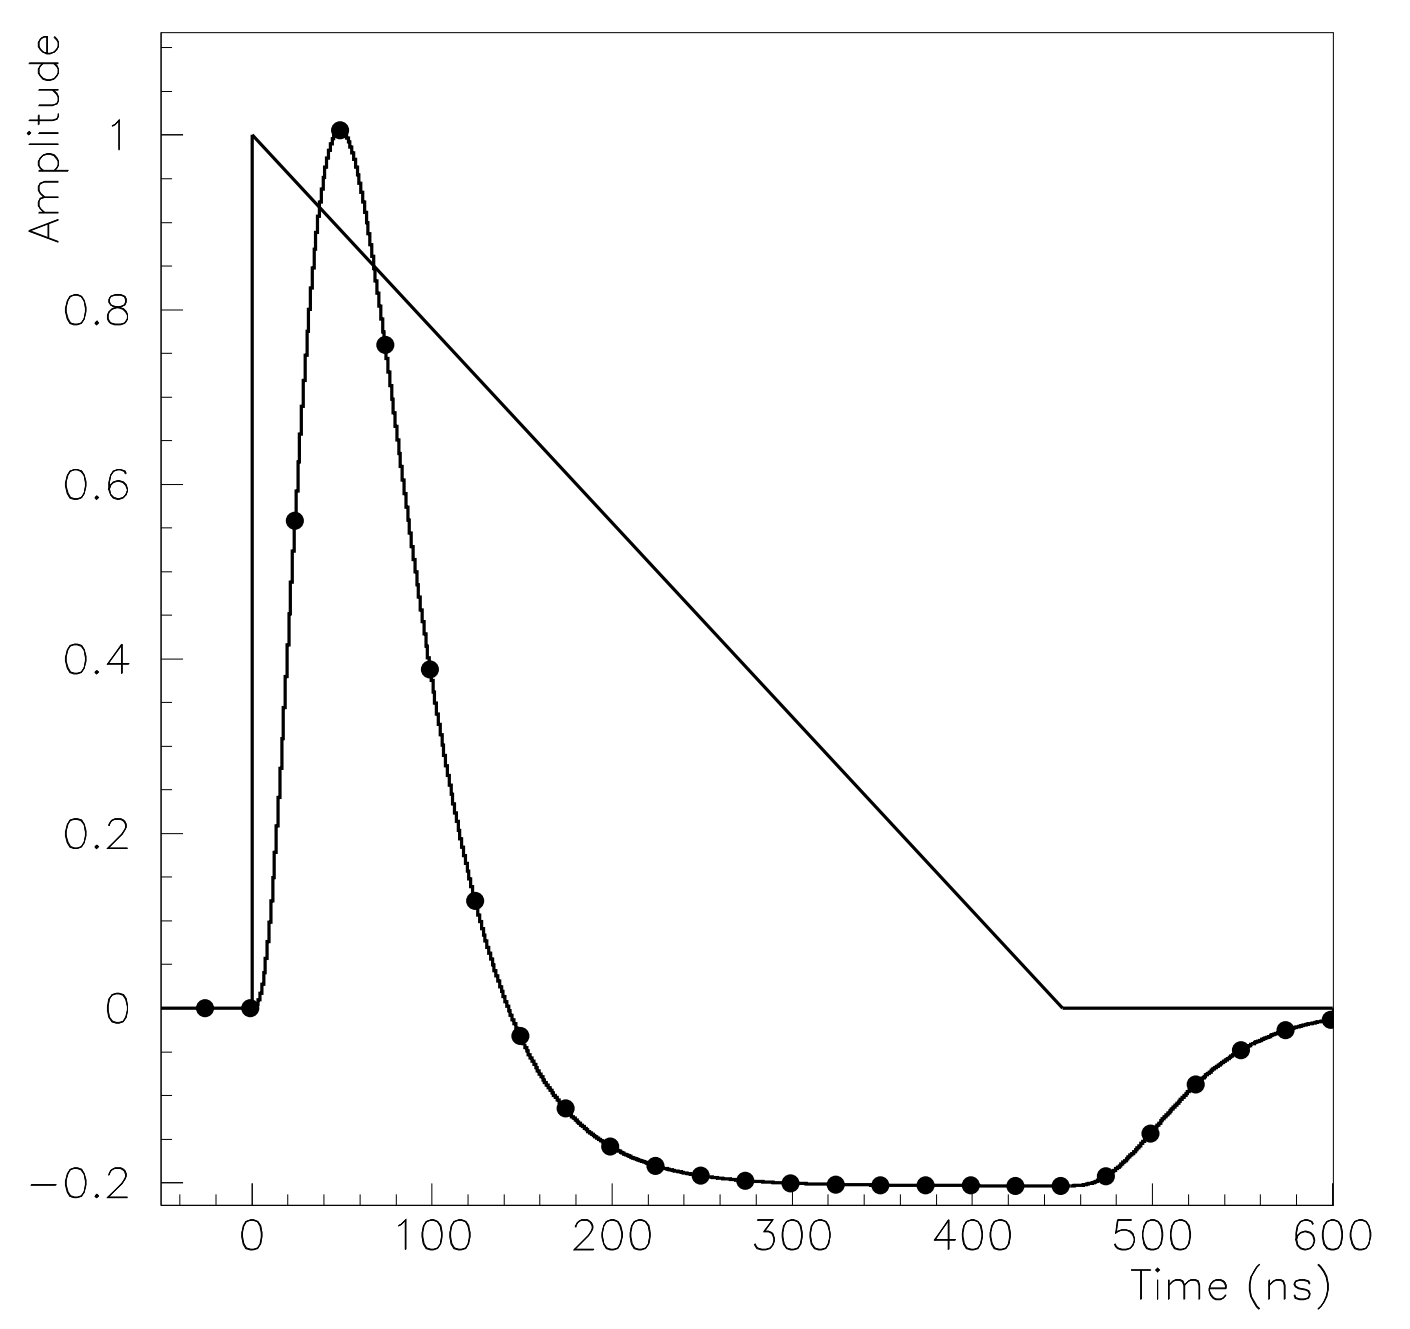
\includegraphics[width=0.5\columnwidth]{figures/Detector/LArPulse.png}
	\caption{LAr Calorimeter pulse shape as produced in the EM barrel before and after shaping.  The dots represent the 25\,ns spacing used in the pulse sampling and digitization.\cite{LArDQ}
	}
	\label{fig:LArPulse}
\end{figure} 

\begin{figure}[]
	\centering
	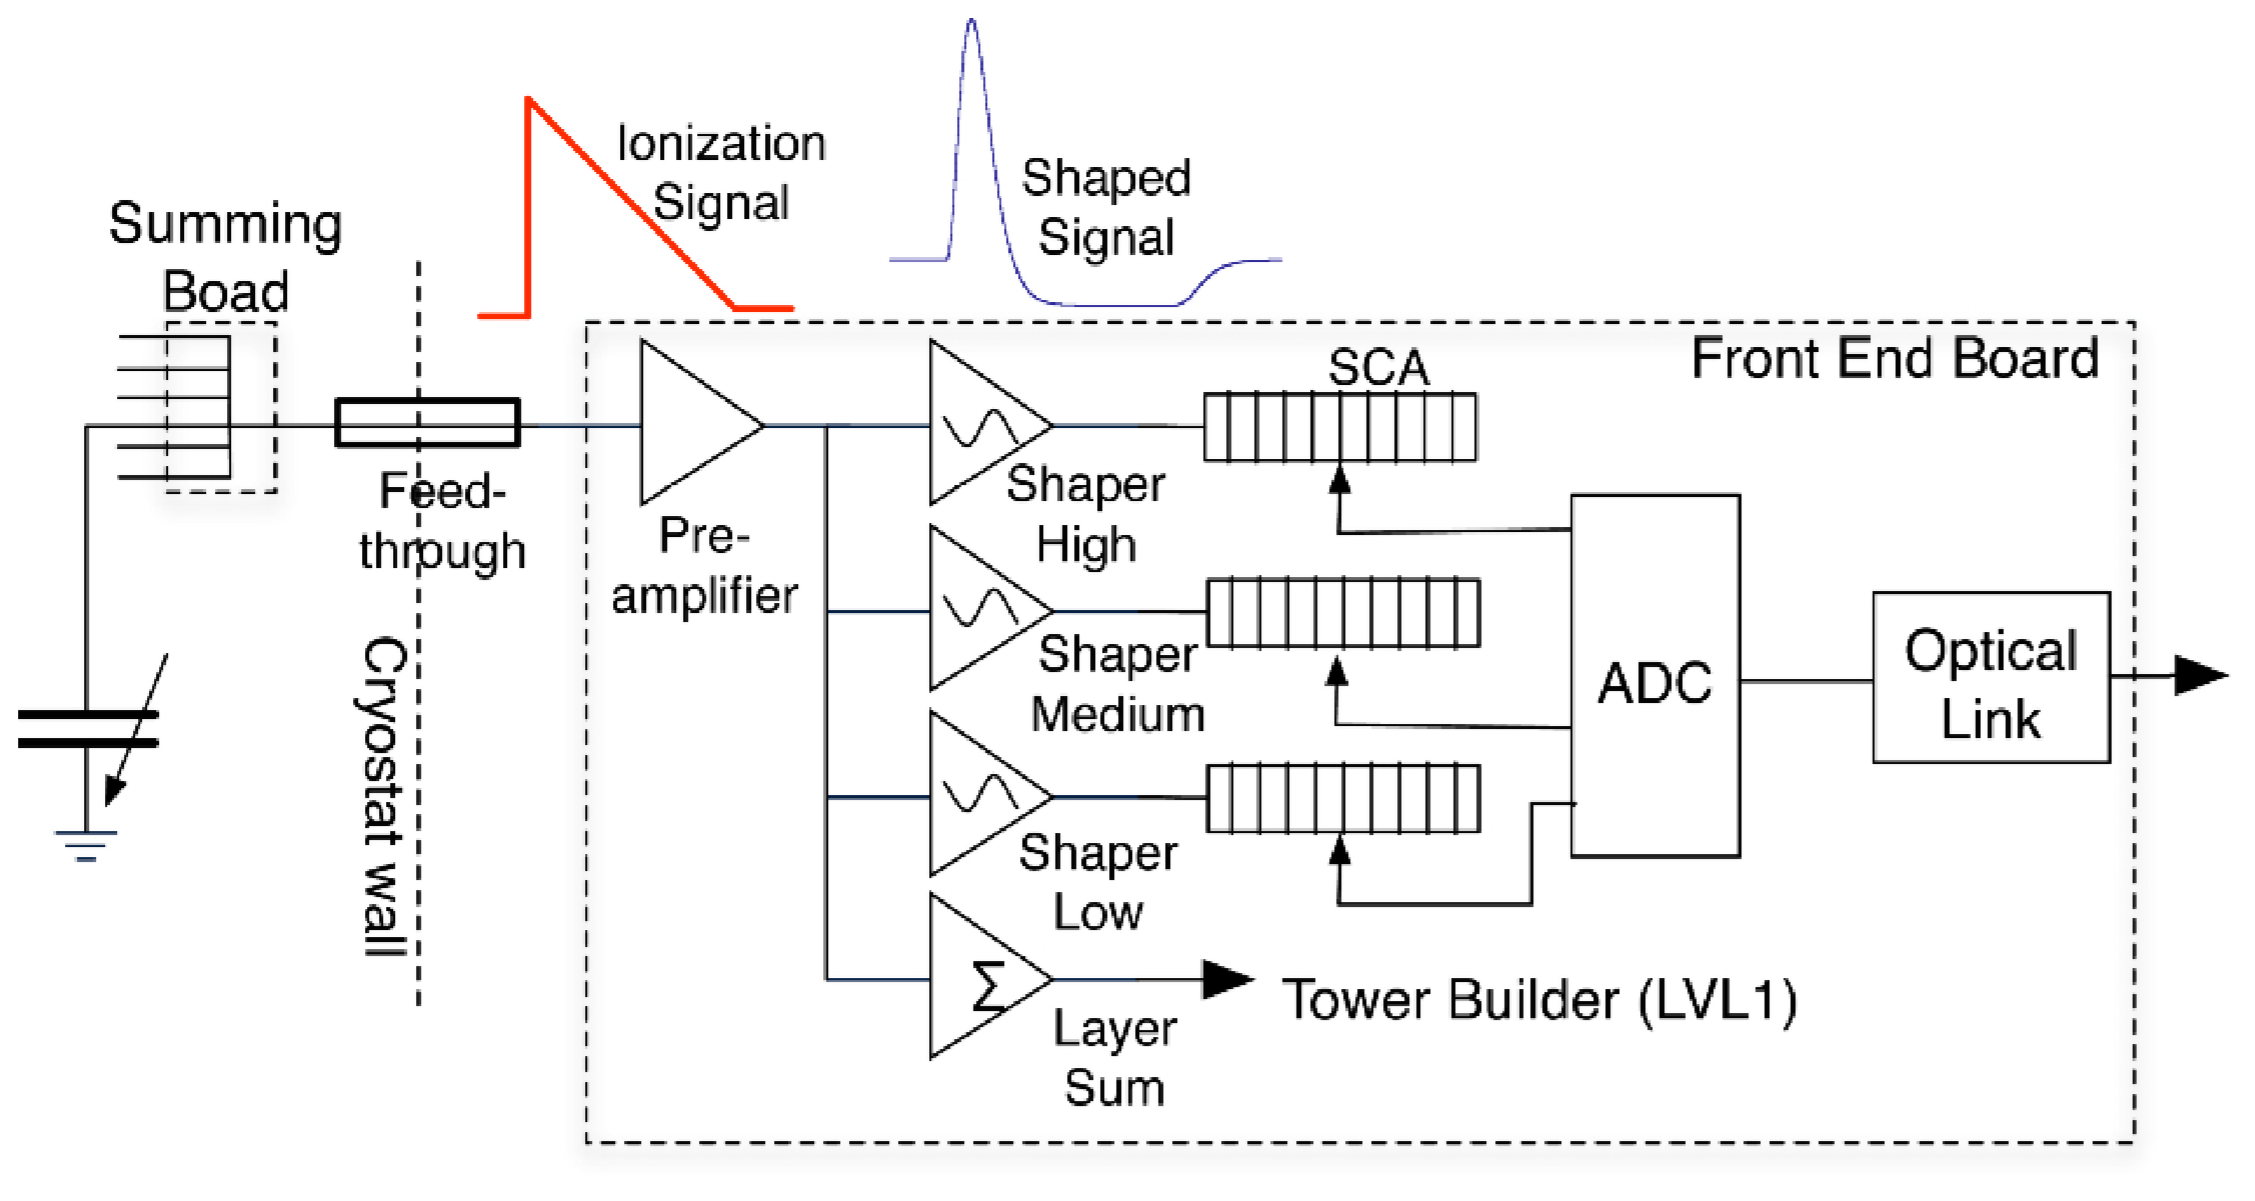
\includegraphics[width=0.8\columnwidth]{figures/Detector/LArReadout.png}
	\caption{The ATLAS LAr Calorimeter front-end system in Run 2, along with the connections to the L1 trigger and readout systems.\cite{LAr_Performance}
	}
	\label{fig:LArOverview}
\end{figure} 

If the event is selected by the L1 trigger system, a Level-1 accept is sent which instructs the board to read out the samples for the corresponding bunch crossing from the SCA where they are digitized by a 12-bit analog-to-digital converter (ADC).  The same gain is used for all channels to reduce any possible systematic effects, and the highest gain which does not saturate a channel is chosen, allowing for the highest possible granularity based on the energy deposited.  The digitized samples are then temporarily stored in memory on the FEB before being sent across optical links to the read-out driver (ROD).


\section{Energy Summing and Triggering Path}
\label{sec:TriggerPath}

Parallel to this process, each set of four calorimeter channels on the FEB is passed to a linear mixer where they are summed together, and the resulting pulse is shaped in the same manner as the individual channels.  Each FEB only processes channels from a single layer of the calorimeter, as different layers can have very different pulse shapes and delays.  The resulting pulse is then sent to a neighboring Tower Builder Board (TBB) which sums together the four layers of the calorimeter (presampler, front, middle, back) into a single pulse.  To do this, it first equalizes the widths of the pulses from the different layers, adjusts the delay for each layer depending on cable length and time-of-flight in the calorimeter, and equalizes the relative gains of the different layers, before finally adding them together into the final pulse.  Additionally, the energy scale is converted from raw energy to transverse energy, the quantity used for most trigger measurements.

These sums are the objects used by the L1 system and are known as trigger towers.  In the central part of the calorimeter the trigger towers cover an area of $0.1\times0.1$ ($\eta\times\phi$), with the EM and hadronic layers each as their own distinct tower.   In the forward regions of the calorimeter the towers become $0.2\times0.2$ ($2.5<|\eta|<3.2$) and $0.4\times0.4$ ($3.2<|\eta|$).

\section{The Level-1 Calorimeter System}

Analog trigger tower signals from the calorimeter systems are sent off detector to the USA15 cavern adjacent to ATLAS to the Level-1 Calorimeter system for further processing.  Signals are send via twisted-pair cables which are routed through special holes between the detector cavern and the trigger system to minimize the latency of the system. The L1Calo system is described in detail in Ref.~\cite{L1Calo_Run1} and the changes for Run 2 in Ref.~\cite{L1Calo_Run2}; the processes most relevant for jet triggering are summarized here.

\begin{figure}[]
	\centering
	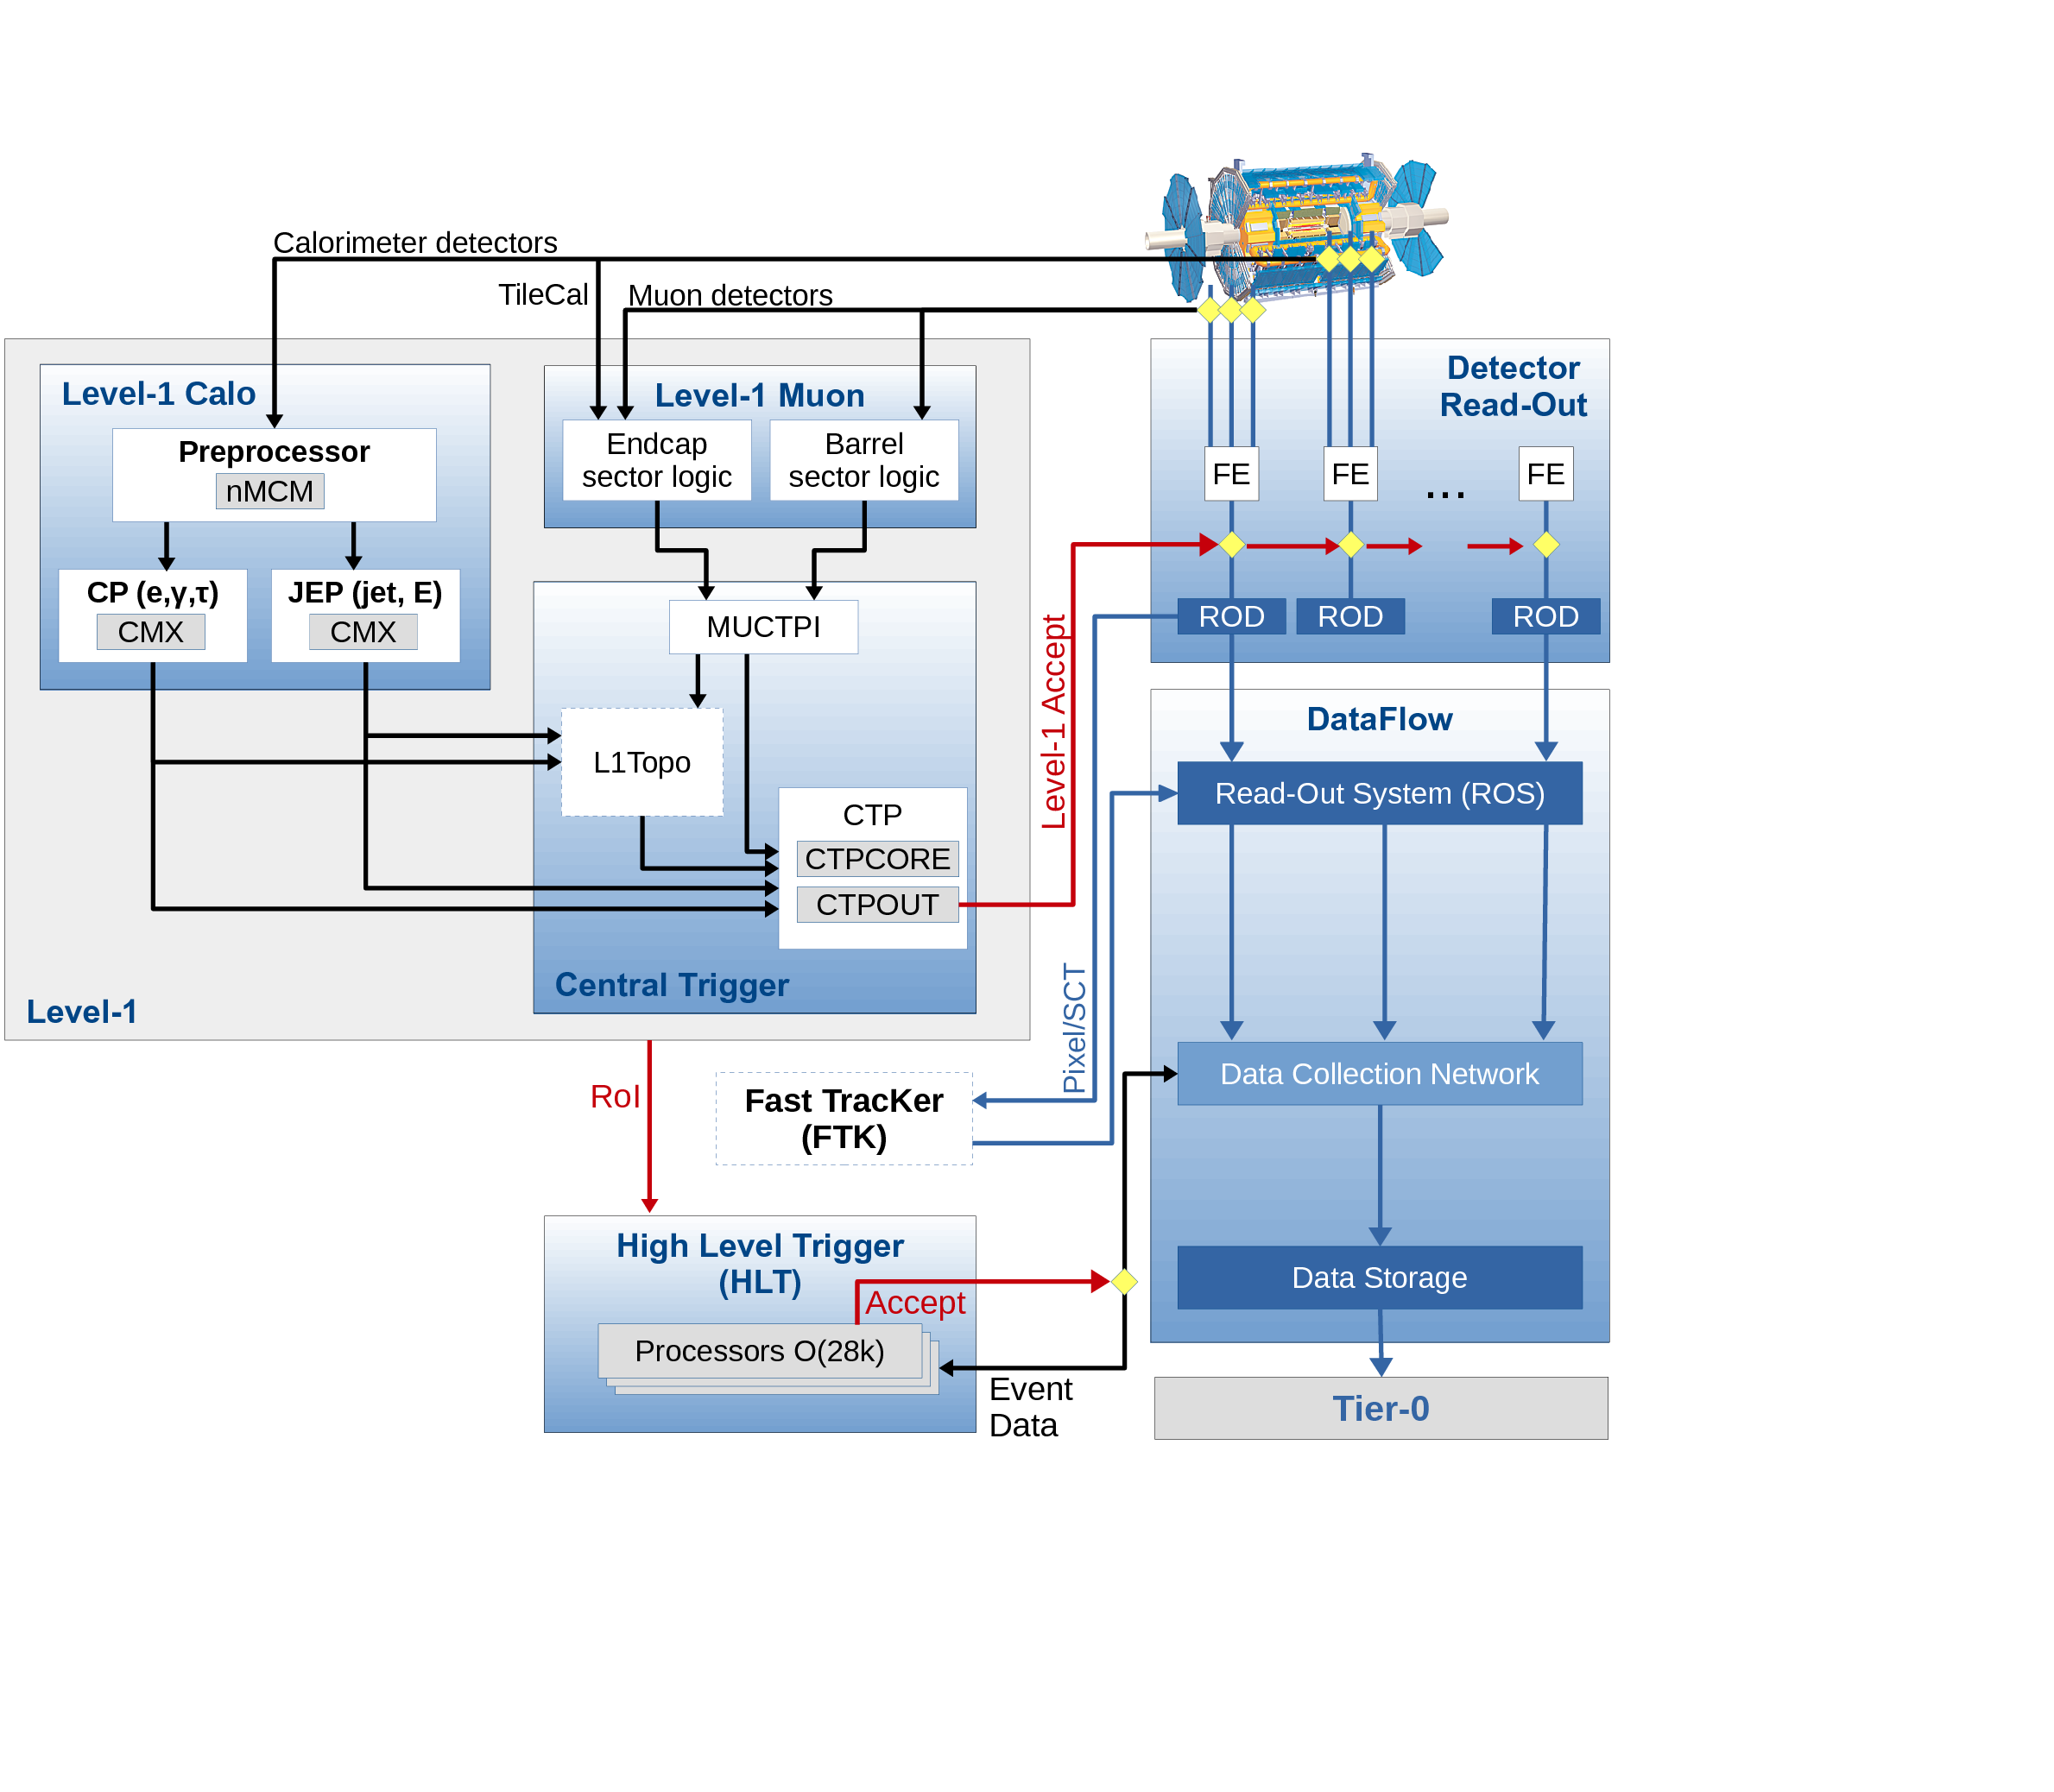
\includegraphics[width=0.8\columnwidth]{figures/Detector/TriggerOverview.png}
	\caption{The ATLAS trigger and data acquisition system in Run 2.  L1Topo was being commissioned in 2015. \cite{L1Calo_Run2}
	}
	\label{fig:TriggerOverview}
\end{figure} 

\subsection{Receiver and PreProcessor Module}
\label{sec:L1Calo}

Their first stop are the L1Calo receivers which apply an $|\eta|$-dependent gain adjustment to equalize the gain across the calorimeter, as well as to convert the hadronic towers from the tile calorimeters from energy to transverse energy.  These signals are then sent to the PreProcessor Module (PPM) which handles the digitization of the calorimeter pulses as well as bunch crossing identification and the final calibration of the trigger towers before their use in the trigger identification algorithms.

Pulses are digitized by a flash-ADC with 10-bit precision, giving quarter-GeV steps and a saturation value of around 250\,GeV for a single tower.  For standard operation 5 samples, spaced by 25\,ns, are read out, though this number can be configured for special runs.  This information is used to understand the pulse shape and to apply the Bunch Crossing Identification(BCID) logic.  To compensate for the different arrival times of each trigger tower due to varying cable lengths between the detector sections and the L1Calo system, the PPM also includes programmable delays in 1\,ns steps to synchronize all of the trigger tower data.  Trigger tower pulses have rise times of approximately two bunch crossings, and as such the pulses from consecutive bunch crossings overlap each other.  To make sure that signals are associated with the correct bunch crossing, two different identification methods are used depending on the energy in a given tower.

For standard, unsaturated signals, the pulse is run through an auto-correlation filter to sharpen the pulse above the background noise level.  This is done by multiplying the five samples by individual coefficients and summing result.  Each section of the calorimeter has varying coefficients due to differences in pulse shape, but the general structure is to multiply by large coefficients for the central samples, and have small or negative coefficients for the samples further away in time.  This sum is then compared to the values obtained for the previous and following bunch crossings; if this value is a local maximum in time, then it is considered to be the peak of the pulse and it is assigned to that bunch crossing.

In the case of saturated signals, the peak is estimated by inspecting the behavior of the leading edge of the pulse and comparing it against predetermined low and high thresholds to determine where the peak is located.  For pulses with only one saturated sample the peak is simple enough to determine; for pulses with multiple saturated samples the peak is either the first or second saturated sample.

It is important to note that the BCID logic does not select an algorithm based on whether or not the pulse is saturated, but rather both algorithms run in parallel for all pulses.  In the case that the two algorithms point to different bunch crossings, the earlier of the two peaks is the one that ends up being used as the second peak falls into the simple dead time after the Level-1 Accept (L1A) from the saturated tower.  The L1A is guaranteed because a saturated trigger tower is set to the maximum possible energy in each step of the jet algorithm, and will therefore trigger several different L1 jet algorithms.

If a pulse is found to peak in a given bunch crossing the result of the filter sum is sent to a look-up table to extract the final transverse energy which is used in the trigger algorithms.  This information is sent as an 8-bit value from 0-255\,GeV; saturated towers are assigned to the maximum possible energy, and towers which do not correspond to the peak of a pulse are set to zero.  Following this step groups of 4 towers are summed to form $0.2\times0.2$ ($\eta\times\phi$) regions which are used in the Jet/Energy-sum Processor, with the sums now having a maximum value of 511\,GeV.  If any of the towers were saturated in the previous sum, these towers are also set to their maximum value.

The PPM also handles the dynamic pedestal correction, a new addition in Run 2.  For each bunch crossing in the machine, and for each channel, the PPM keeps a running value of the average filter output run over many bunch crossings.  This gives an approximation of the average noise and pileup energy for a given tower, and this value is then subtracted from the peak finder filter output to give a corrected value which is translated to an energy via the look-up table.  This bunch-dependent method is responsible for keeping L1 missing energy trigger rates in check with the increase in luminosity by cutting down on the amount of triggers that happen earlier in the bunch train; the pulse behavior in the beginning of a bunch train is different because it lacks the overlaid pulses and undershoots that bunches later in the train encounter.  The magnitude and effect of this pedestal correction is shown in Figure~\ref{fig:Pedestal}.  The correction spikes at the beginning of each bunch train and tapers off after the first few bunches.

\begin{figure}[h!]
	\centering
	\subfloat[]{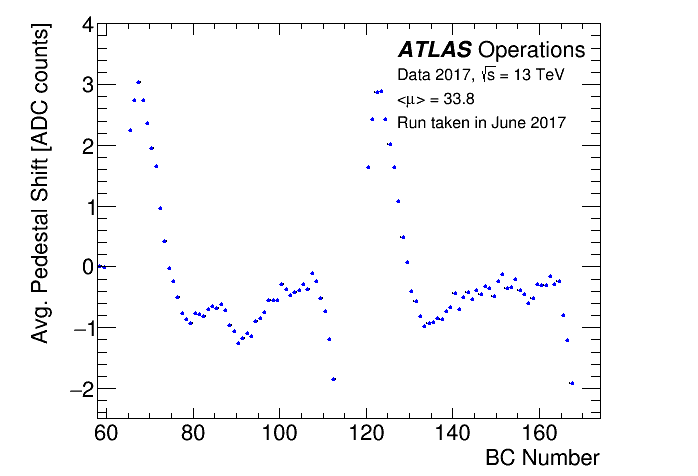
\includegraphics[width=0.50\columnwidth]{figures/Detector/L1CaloPedestal.png}\label{subfig:L1CaloPedestal}}
	\hspace{0.1\textwidth}%
	\subfloat[]{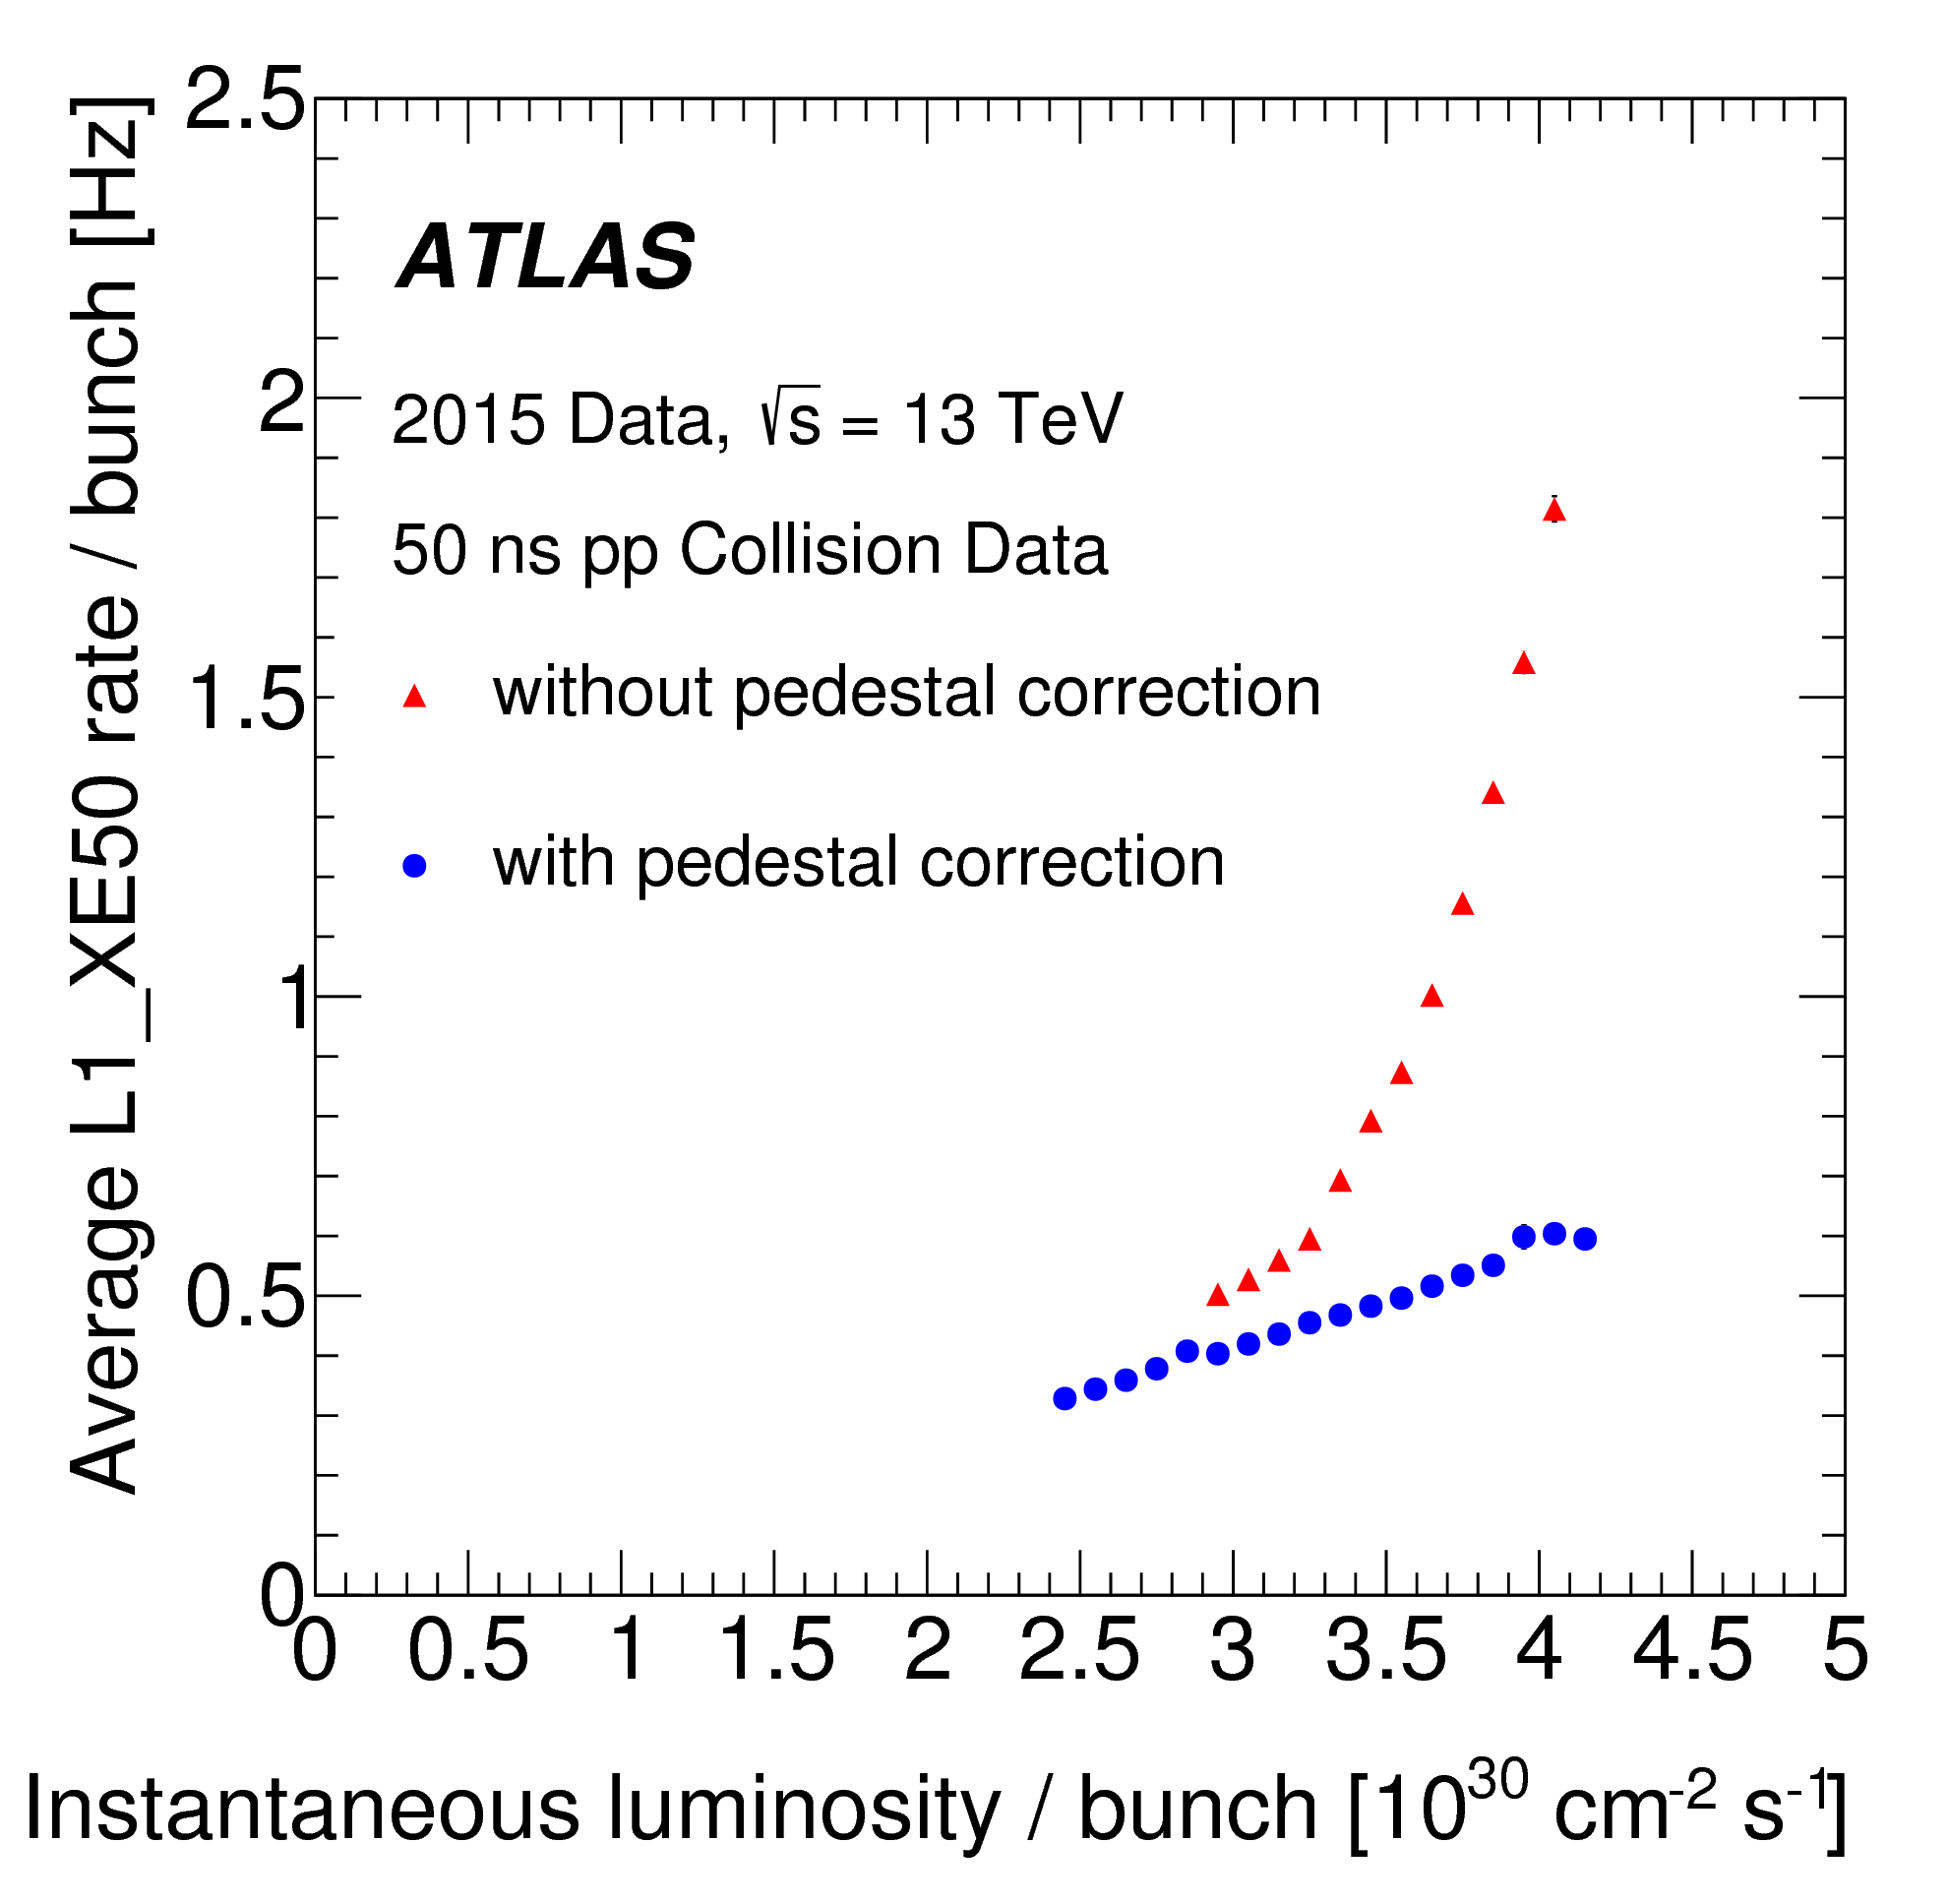
\includegraphics[width=0.35\columnwidth]{figures/Detector/Pedestal.png}\label{subfig:Pedestal}}
	\caption{(a) The average pedestal correction per trigger tower as a function of the Bunch Crossing ID (BCID) in the Electromagnetic Barrel partition of the LAr calorimeter during a 2017 run.  1 ADC count is approximately equal to 0.25\,GeV of transverse energy in a single tower.\cite{L1CaloPedestal} (b) The per-bunch trigger rate for the L1 missing transverse momentum trigger with a threshold of 50\,GeV (L1\_XE50) as a function of the instantaneous luminosity per bunch. The rates are shown with and without pedestal correction applied. \cite{L1Calo_Run2} 
	}
	\label{fig:Pedestal}
\end{figure} 

\subsection{Cluster and Jet/Energy-Sum Processors}

The Cluster Processors (CP) and Jet/Energy-Sum Processors (JEP) handle the calculations for detecting physics objects, with the CP handling electron/photon and tau algorithms while the JEP handles jets and missing transverse energy.  The CP handles $0.1\times0.1$ calorimeter data out to $|\eta|<2.5$ while the JEP uses the larger $0.2\times0.2$ towers out to $|\eta|<3.2$ and the full calorimeter for the missing transverse energy algorithms.  The CP uses the separate EM and hadronic tower information for hadronic isolation algorithms, but in the JEP this is unnecessary and so the EM and hadronic trigger towers are added together to create the $0.2\times0.2$ jet elements which are used in the trigger algorithms with transverse energy values up to 1023\,GeV with 1\,GeV granularity.  If either the EM or hadronic towers are set to their maximum value indicating saturation, then the resulting jet element is also set to its maximum value.

The L1 jet algorithm uses a rectangular sliding window of $4\times4$ jet elements ($0.8\times0.8$ in $\eta\times\phi$) which moves along the whole detector and looks for windows with a transverse energy above a given jet threshold.  The algorithm first creates $2\times2$ core sums which are required to be local maxima; those that pass then have the transverse energy of the full window compared against a set of energy thresholds.  The jet trigger algorithm window is shown in Figure~\ref{fig:JetWindows}; the original L1Calo designed allowed for algorithms which used the same sliding window and local maxima technique but with smaller jet areas of $2\times2$ or $3\times3$ jet elements, however these are not currently used for any jet triggers.  All jet candidates are saved as Trigger Objects (TOBs) which carry the jet transverse energy as well as the $\eta-\phi$ position of the core, and are passed to the L1Topo system for use in topological algorithms.  In the case of a Level-1 accept, the entire calorimeter is read out and used for jet reconstruction in the HLT.

\begin{figure}[h!]
	\centering
	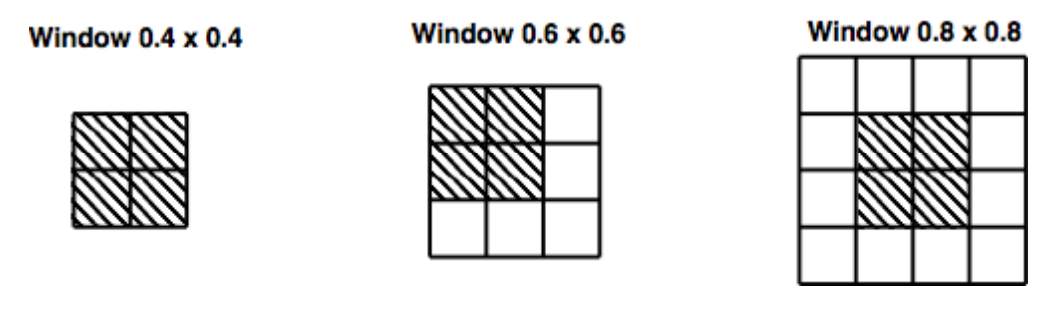
\includegraphics[width=0.7\columnwidth]{figures/Detector/JetWindows.png}
	\caption{Jet trigger algorithm windows using $0.2\times0.2$ ($\eta\times\phi$) jet elements with the local maxima cores shaded in.  Only the $0.8\times0.8$ window is currently used for jet finding.\cite{L1Calo_Run1}
	}
	\label{fig:JetWindows}
\end{figure} 



\section{High-Level Trigger}
\label{sec:Topoclustering}
The High-Level Trigger has much longer time to process an event (500\,ms compared to 2.5\,$\mu$s for Level-1) as well as access to full-granularity information from the calorimeter.  This allows the HLT to use much more precise, and computationally expensive, algorithms to calculate jet energies at levels very close to offline performance.  Groups of calorimeter cells with significant deposits of energy are grouped together using the technique of topological cell clustering, or topoclustering, which is described in Ref.~\cite{Topoclustering} and summarized here.

Topoclustering attempts to create groups of topologically connected calorimeter cells which have signals above the background of the combined noise from electronics and the background pile-up in an event.  To do this, the energy in a given cell is compared against an estimated average noise value assigned it using the ratio in Equation~\ref{eq:Topocluster}.

\begin{equation}
\varsigma^{EM}_{cell} = \frac{E^{EM}_{cell}}{\sigma^{EM}_{noise,cell}}
\label{eq:Topocluster}
\end{equation}

Topoclustering proceeds using a 4-2-0 algorithm, corresponding to the values of $|\varsigma^{EM}_{cell}|$ used for each step of the clustering algorithm.  This particular configuration was found to provide the best energy resolution for pions in test beam data.\cite{Topoclustering420}  Topoclusters are seeded by cells which have energies at least four standard deviations larger than the noise.  From these seeds, all neighboring cells are checked to see if they are more than two sigma above their noise value; if so they are added into the cluster.  Neighboring cells are checked in three dimensions, so adjacent cells in the same layer are checked as well as cells overlapping the previous cell in the $\eta-\phi$ plane in an adjacent layer.  This checking procedure is applied iteratively, so all neighbors to this first layer are checked as well, repeating until there are no more contiguous cells above two times their noise value.  Finally, a perimeter layer using all cells regardless of energy is added to the cluster.

The goal of topocluster creation is to suppress the effects of noise and pileup by requiring highly-significant energy deposits to create and expand clusters, but it also allows for softer radiation to be captured in the perimeter step to maximize the amount of jet energy captured.  The final cluster can grow to be very large and encompass a significant portion of the detector depending on the distribution of particles in the event, and so a final splitting step is added to differentiate between close-by particles within the cluster.  This is done by re-clustering the cells included in the current topocluster using all cells which are above a given energy threshold and are also local maxima.\cite{LArTopoclustering}  The clusters are then created in the same manner as before, but only using the cells previously selected, not re-applying the threshold requirement, and not allowing clusters to overlap and merge.  When two or more clusters are adjacent to a cell the energy is split between the two clusters based on their energies and distance from the shared cell.  The final cluster is then kept is the total transverse energy is above a certain cutoff, with 400 MeV used as the threshold for the 2016 data reconstruction.

These topoclusters are what are used as inputs for the HLT jet reconstruction algorithm, which each cluster being treated as a massless four-vector with an energy equal to the sum of all of the cells in the cluster and a location based on the energy-weighted center of the cluster.  Jets are reconstructed using the anti-$k_t$ algorithm~\cite{AntiKt} with radius of $R = 0.4$ for single-jet triggers, and are calibrated using an approximation of the full offline calibration sequence.\cite{L1Calo_Run2}.  If the final jet energy exceeds the given energy threshold for its trigger chain then the event is saved to disk and processed for offline analysis.